
\chapter{Certificado autofirmado SSL}

Vamos a comenzar trabajando en m1, todos los comandos y configuraciones que se van a mostrar a continuación se ralizarán en esta máquina.

Primero creamos la carpeta donde vamos a guardar los certificados \verb|/etc/apache2/ssl| y luego vamos a activar el módulo ssl y relanzamos apache, para lo que ejecutamos los comandos que se muestran en \eqref{ssl_1}.

\begin{figure}[h!]
\begin{center}
\caption{Creación del directorio para almacenar los certificados, instalación del módulo ssl y relanzar apache.}
\label{ssl_1}
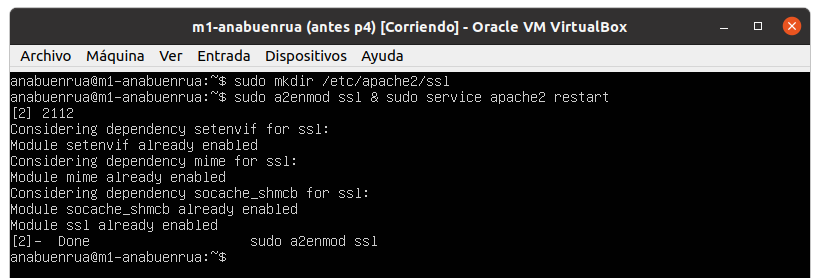
\includegraphics[scale=0.5]{ssl_1b}
\end{center}
\end{figure}

Ahora procedemos a crear los certificados con \verb|ssl|, como se ve en \eqref{ssl_3}.

\begin{figure}[h!]
\begin{center}
\caption{Creación de los certificados con ssl.}
\label{ssl_3}
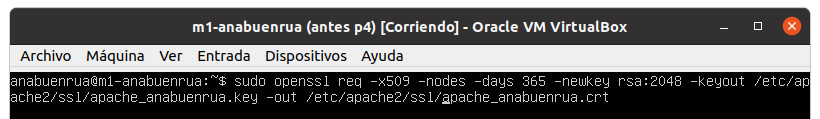
\includegraphics[scale=0.5]{ssl_3}
\end{center}
\end{figure}

En \eqref{ssl_3} hemos usado varios argumentos que explicamos a continuación:

\begin{itemize}
\item \verb|-x509|: Autofirma el certificado.
\item \verb|-days|: Indica que el certificado va a tener 365 días de validez.
\item \verb|-keyout|: Especifica el fichero donde se va a guardar la clave.
\item \verb|-out|: Especifica el fichero donde se va a guardar el certificado.
\end{itemize}

Además, le hemos indicado que la clave es de 2048 bits.

A continuación introducimos los datos que nos piden por línea de comandos, se ve en \eqref{ssl_4}.

\begin{figure}[h!]
\begin{center}
\caption{Introducimos los datos requeridos para la creación del certificado.}
\label{ssl_4}
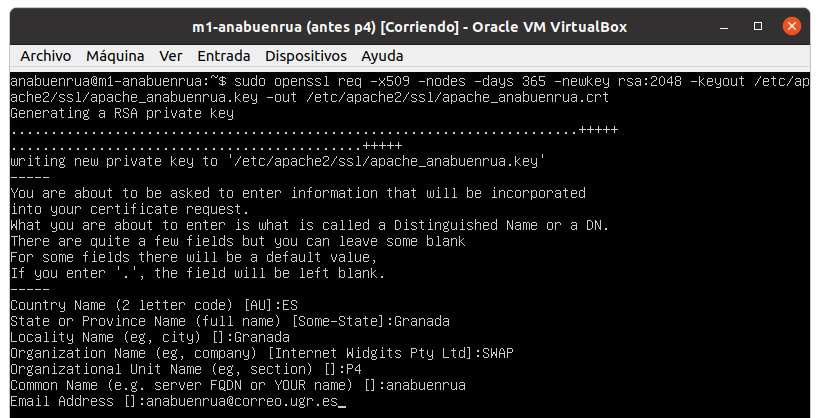
\includegraphics[scale=0.5]{ssl_4}
\end{center}
\end{figure}

\section{Opciones avanzadas}

Como opciones avanzadas, se van a comentar distintos argumentos para generar los certificados con \verb|openssl req|.

\begin{itemize}
\item \verb|-inform DER/PEM| especifica el formato de entrada de los datos.
\item \verb|-outform DER/PEM| especifica el formato de salida de los datos.
\item \verb|-subj /type0=value0/type1=value1/type2=...| permite especificar los datos desde la orden. Las abreviaturas que sustituyen a type0, type1 están predefinidas y pueden consultarse en el manual.
\item \verb|-text| imprime el certificado en forma de texto.
\end{itemize}


\chapter{Apache con certificado SSL}

Para configurar apache para que use el certificado SSL que acabamos de generar, vamos a empezar configurando la ruta de los certificados en apache.

Editamos el archivo \verb|/etc/apache2/sites-available/default-ssl| con la información de nuestros certificados, como se muestra en \eqref{ssla_1}.

\begin{figure}[h!]
\begin{center}
\caption{Archivo /etc/apache2/sites-available/default-ssl.}
\label{ssla_1}
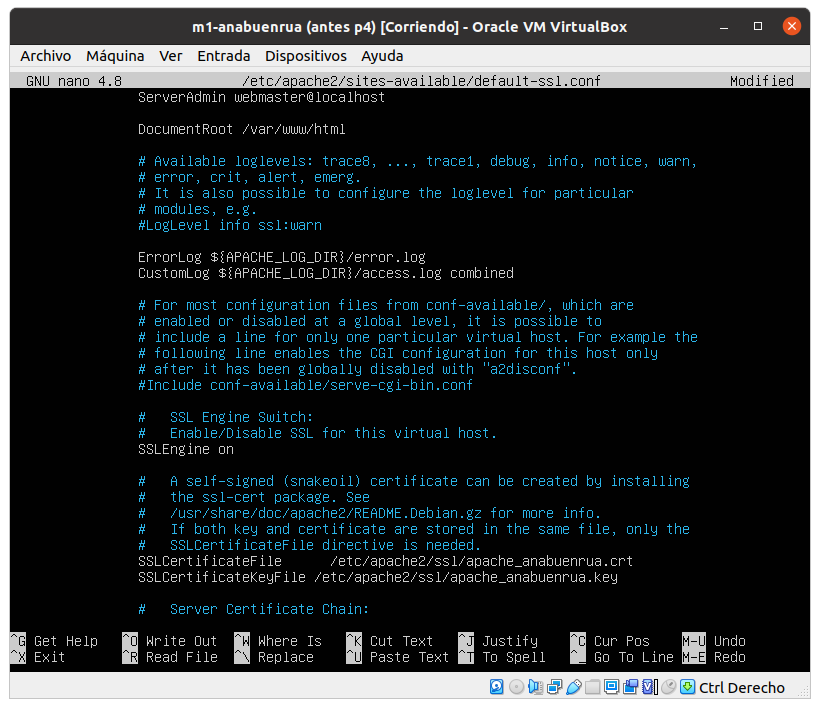
\includegraphics[scale=0.5]{ssla_1}
\end{center}
\end{figure}

Ahora activamos el sitio \verb|deafult-ssl|, para lo que se ejecuta \eqref{ssla_2}.

\begin{figure}[h!]
\begin{center}
\caption{Activación del sitio default-ssl}
\label{ssla_2}
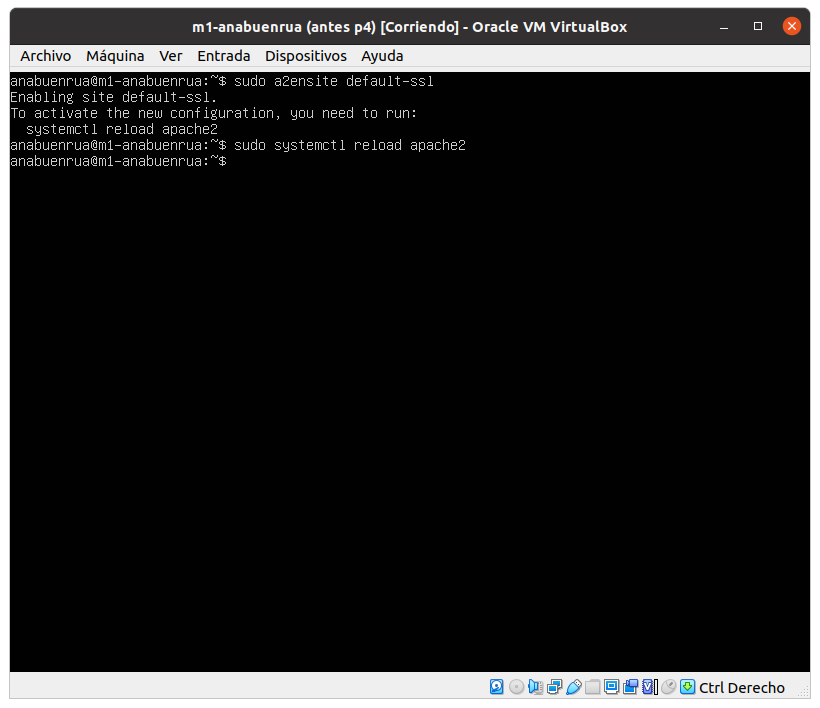
\includegraphics[scale=0.5]{ssla_2}
\end{center}
\end{figure}

Para comprobar que hemos realizado todo correctamente, ahora accedemos a m1 desde el navegador, como en las otras prácticas vamos a acceder a la página \verb|swap.html| usando https.

Nos informa de que la conexión no es segura porque el certificado es autofirmado, pero le damos a continuar de todas formas, como se ve en \eqref{ssla_3}.

\begin{figure}[h!]
\begin{center}
\caption{Aviso de conexión no segura al acceder a m1 desde el navegador.}
\label{ssla_3}
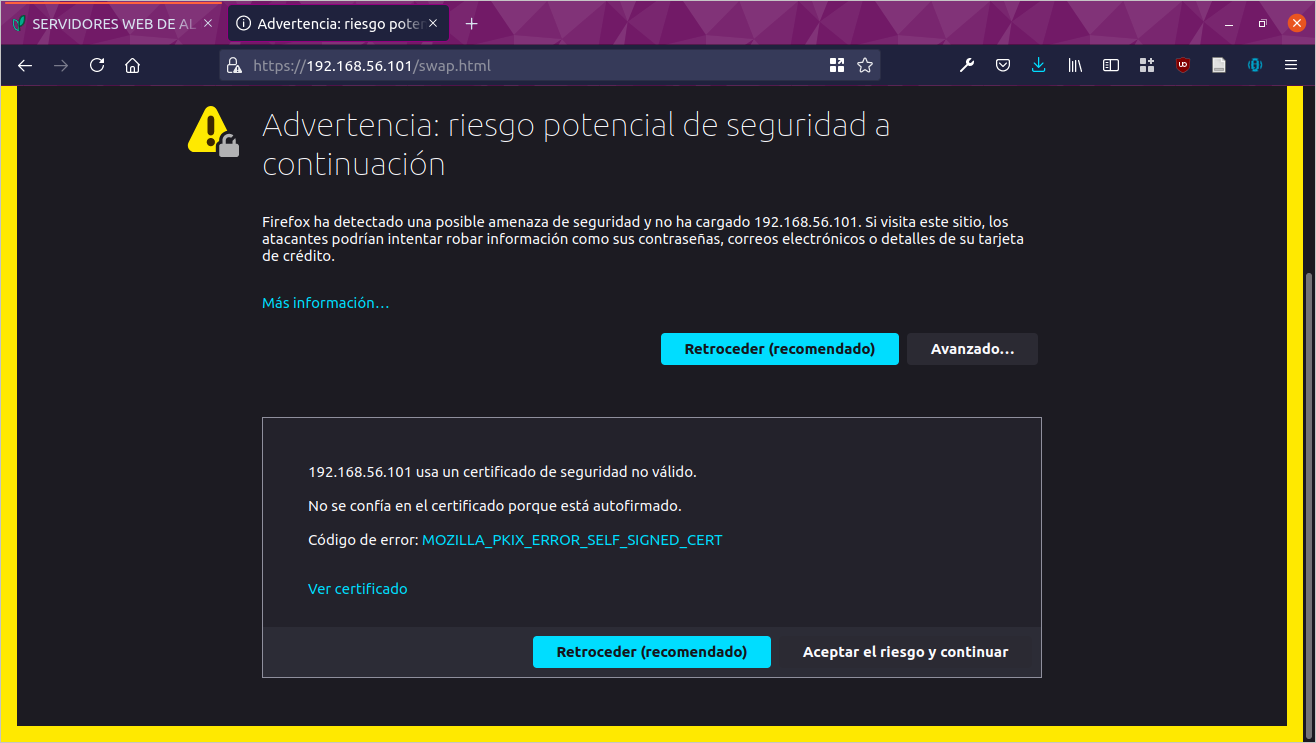
\includegraphics[scale=0.5]{ssla_3}
\end{center}
\end{figure}

Tras el aviso, accedemos a la página, donde vemos ne la parte de la url el candado a la izquierda, aunque tiene una exclamación, indicando de nuevo que el certificado es autofirmado. Esto puede verse en \eqref{ssla_4}

\begin{figure}[h!]
\begin{center}
\caption{Acceso a swap.html de m1.}
\label{ssla_4}
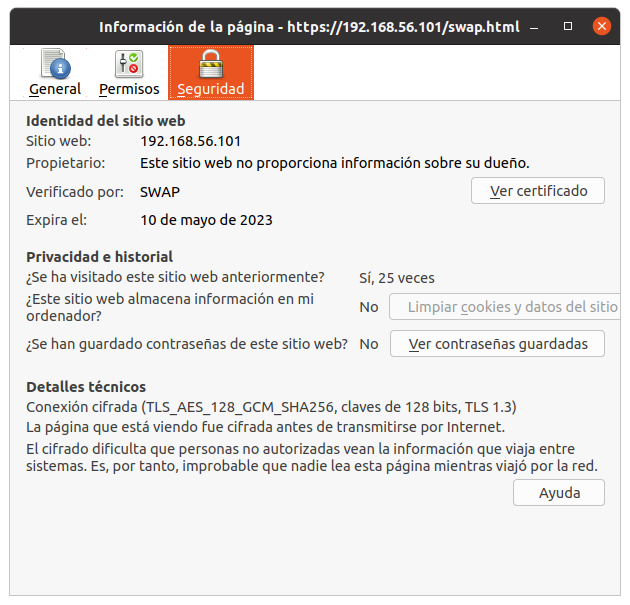
\includegraphics[scale=0.5]{ssla_4}
\end{center}
\end{figure}

Si pulsamos sobre este candado y le damos a más infromación, nos muestra más detalles sobre el certificado, como se muestra en \eqref{ssla_6}.

\begin{figure}[h!]
\begin{center}
\caption{Información del certificado mostrada por firefox.}
\label{ssla_6}
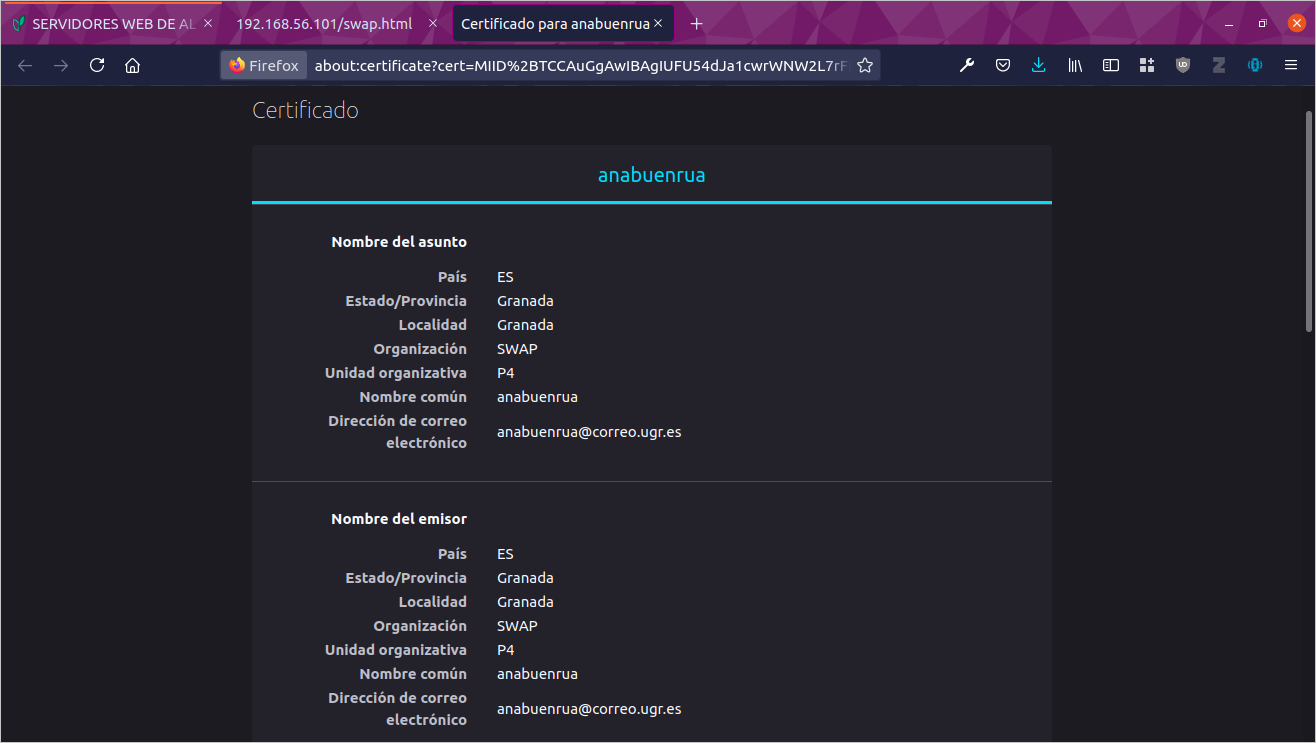
\includegraphics[scale=0.5]{ssla_6}
\end{center}
\end{figure}

Finalmente, vamos a copiar los certificados de m1 en m2, para lo que vamos a usar \verb|scp|.

Para ello, primero creamos el directorio para almacenar los certificados en cada máquina y luego los copiamos mediante \verb|scp|, ejecutando los comandos de \eqref{ssla_8} en m1.

\begin{figure}[h!]
\begin{center}
\caption{Copia de certificados de m1 en m2 mediante scp.}
\label{ssla_8}
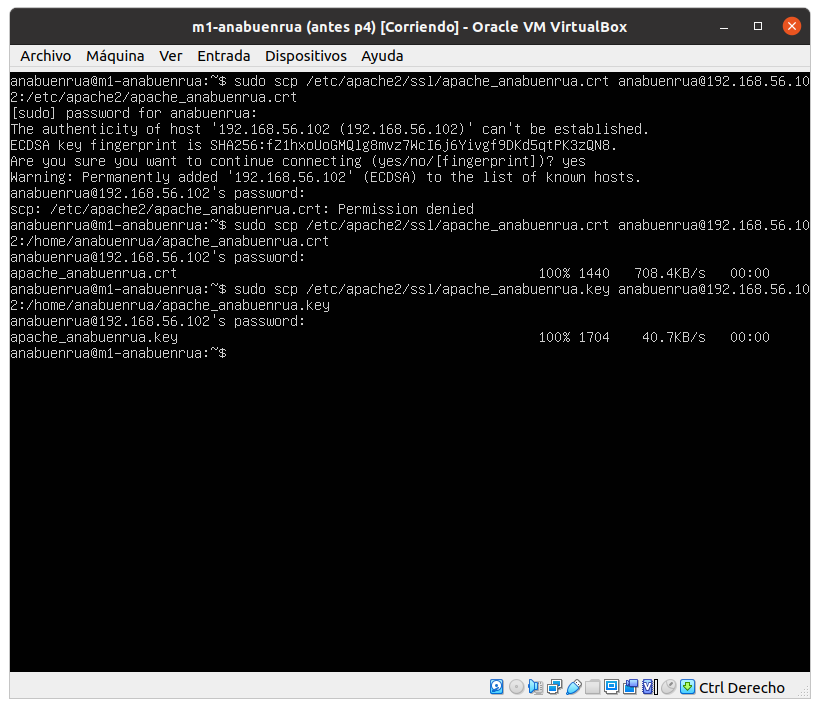
\includegraphics[scale=0.5]{ssla_8}
\end{center}
\end{figure}

Ahora movemos los ficheros al mismo directorio que en m1 y repetimos el proceso para activar el módulo ssl, configuramos el archivo \verb|/etc/apache2/sites-available/default-ssl|, activarlo y reiniciamos apache, de forma análoga a como lo hemos hecho en m1, y comprobamos que funciona en \eqref{ssla_9}

\begin{figure}[h!]
\begin{center}
\caption{Comprobación del funcionamiento correcto de m2 con los certificados.}
\label{ssla_9}
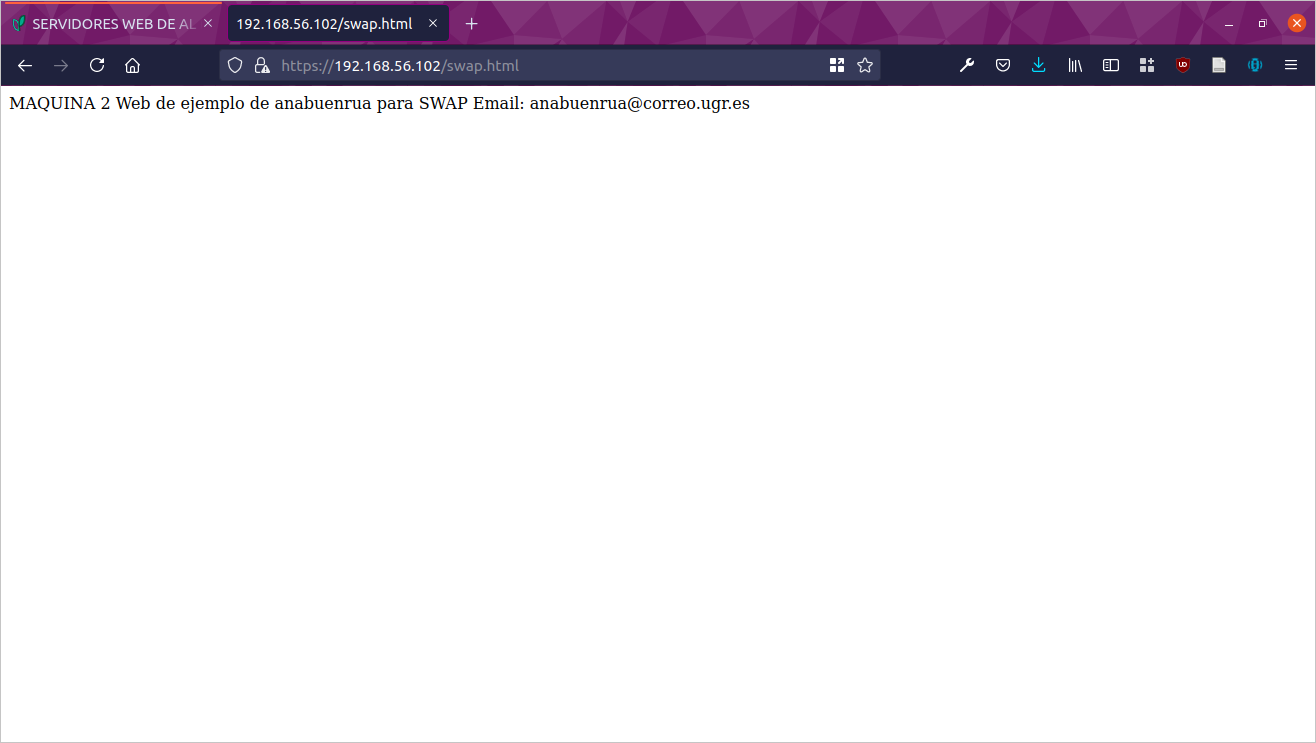
\includegraphics[scale=0.5]{ssla_9}
\end{center}
\end{figure}


\section{Opciones avanzadas}

Podemos obtener el certificado mediante openssl, para ello he usado mi ordenador anfitrión como se ve en \eqref{ssla_7}.

\begin{figure}[h!]
\begin{center}
\caption{Obtención del certificado mediante openssl.}
\label{ssla_7}
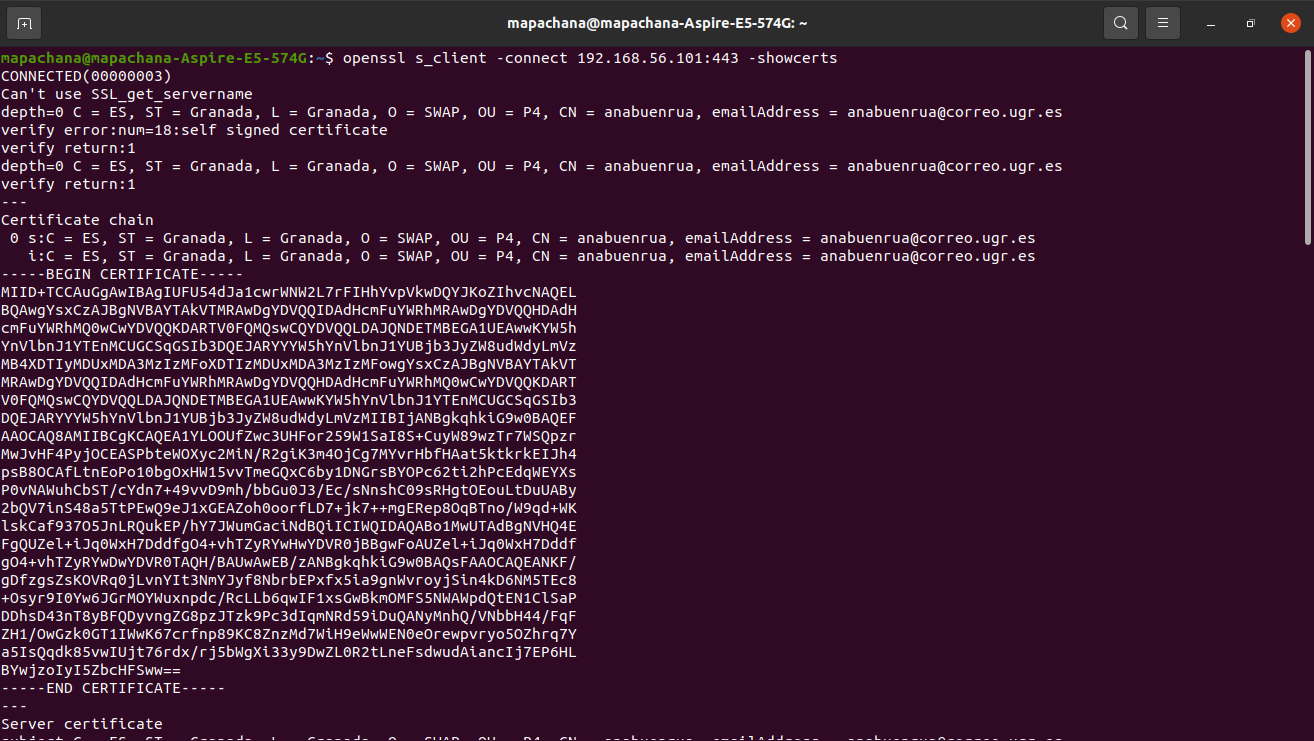
\includegraphics[scale=0.5]{ssla_7}
\end{center}
\end{figure}

Y comprobamos que nos muestra el certificado.

Además, se pueden añadir otras opciones de apache con \verb|SSLOptions +opcion|.

También se puede activar la redirección para que toda conexión http la redirija a ser https:

\begin{verbatim}
<VirtualHost *:80>
        // Cosas

        Redirect "/" "https://your_domain_or_IP/"

        //Más cosas
</VirtualHost>
\end{verbatim}

\chapter{Nginx como balanceador para peticiones HTTPS}

Para configurar nginx con los certificados ssl, comenzamos copiando los ficheros de m1 a m3 mediante scp, se puede ver en \eqref{nginx_1}.

\begin{figure}[h!]
\begin{center}
\caption{Copia de certificados de m1 a m3 mediante nginx.}
\label{nginx_1}
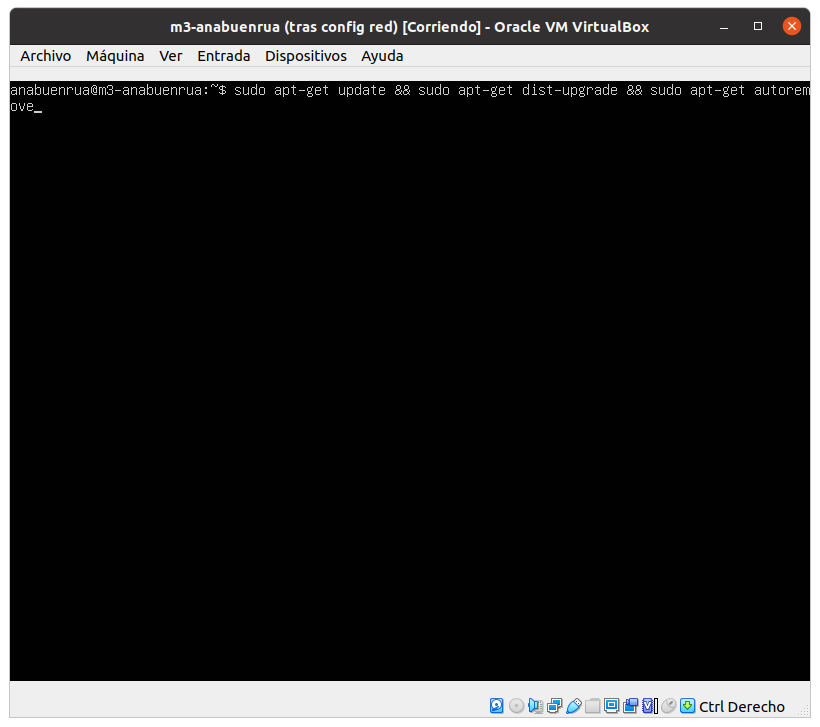
\includegraphics[scale=0.5]{nginx_1}
\end{center}
\end{figure}

Creamos una carpeta ssl como anteriormente y movemos ahí los certificados copiados.

Ahora editamos el fichero de configuración de nginx \verb|/etc/nginx/conf.d/default.conf| añadiendo un servidor nuevo como se muestra en \eqref{nginx_2}.

\begin{figure}[h!]
\begin{center}
\caption{Fichero /etc/nginx/conf.d/default.conf.}
\label{nginx_2}
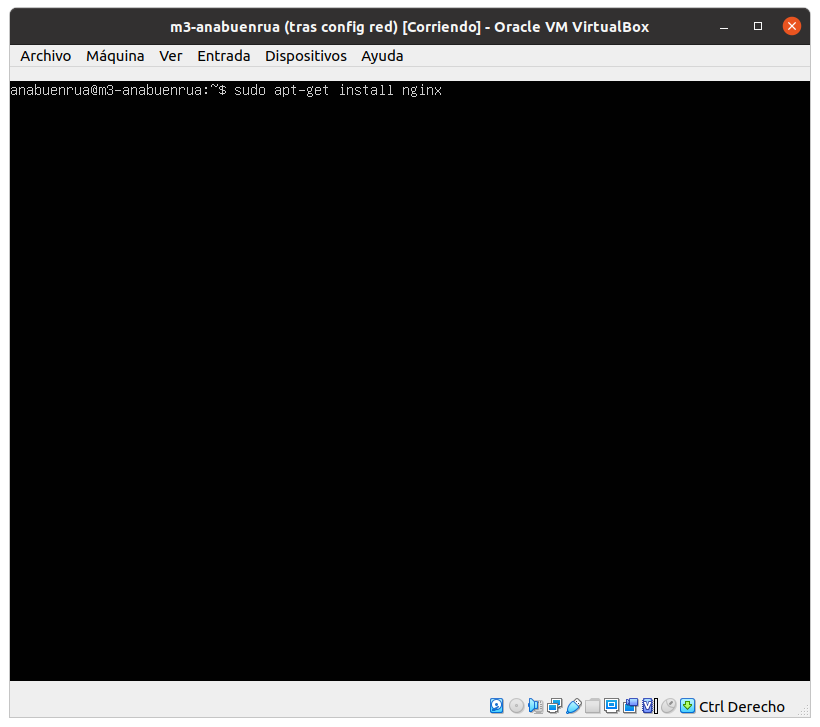
\includegraphics[scale=0.5]{nginx_2}
\end{center}
\end{figure}

Relanzamos nginx con \verb|sudo systemctl restart nginx| y comprobamos que podemos acceder al balanceador por https, como se ve en \eqref{nginx_3}.

\begin{figure}[h!]
\begin{center}
\caption{Acceso a m3 por https.}
\label{nginx_3}
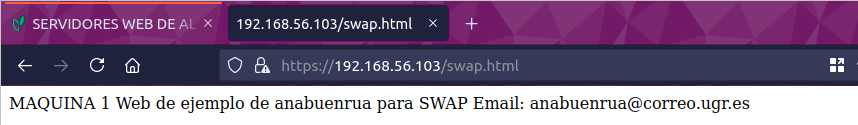
\includegraphics[scale=0.5]{nginx_3}
\end{center}
\end{figure}

\section{Opciones avanzadas}

Como configuraciones adicionales para nginx se pueden usar varias directivas dentro del archivo de configuración \verb|/etc/nginx/conf.d/default.conf|:

\begin{itemize}
\item \verb|ssl_protocols <lista de protocolos>|. Su función es indicar que las conexiones por SSL y TLS que se van a establecer deben ser compatibles con las de la lista de protocolos indicada. Por ejemplo, SSLv2, TLSv1 o TLSv2.
\item \verb|ssl_ciphers <lista de protocolos>|. Su función es, de análogamente a \verb|ssl_protocols|, limitar las conexiones a aquellas compatibles con los sistemas cifrados listados.
\end{itemize}

\chapter{IPTABLES}

Comprobamos que el cortafuegos iptables está ya instalado en todas las máquinas con \verb|iptables --version|.

Vamos a comenzar creando un script para aceptar todo el tráfico, ya que es la restricción más amplia al no tener ninguna y aceptar cualquier petición.

Después, iremos añadiendo otras reglas más específicas para restringir el tráfico, recordando siempre que la última regla introducida tiene prioridad sobre las anteriores.

Creamos un directorio en cada máquina \verb|/home/anabuenrua/scripts_iptable| para almacenar todos los scripts.

En primer lugar realizamos el script para permitir todo el tráfico, para ello creamos el script \eqref{iptable_1} en m1.

\begin{figure}[h!]
\begin{center}
\caption{Script de iptables para admitir todo el tráfico.}
\label{iptable_1}
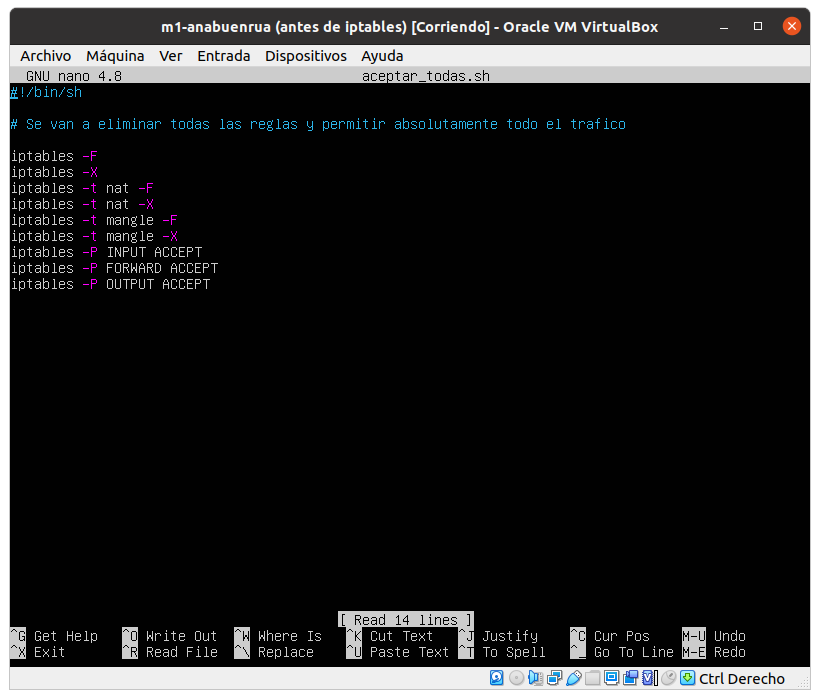
\includegraphics[scale=0.5]{iptable_1}
\end{center}
\end{figure}

Lo ejecutamos mediante \verb|sudo bash aceptar_todas.sh| y comprobamos que podemos seguir accediendo normalmente a ella, como por ejemplo mediante ping, como se ve en \eqref{iptable_2}.

\begin{figure}[h!]
\begin{center}
\caption{Ping a m1 tras configuración básica de aceptar todas las peticiones.}
\label{iptable_2}
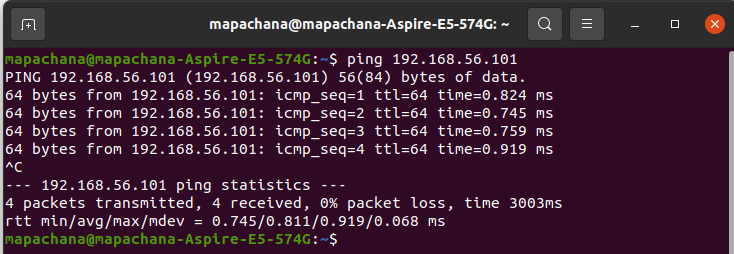
\includegraphics[scale=0.5]{iptable_2}
\end{center}
\end{figure}

Ahora, escribimos un script para denegar todo el tráfico, que se muestra en \eqref{iptable_3}.

\begin{figure}[h!]
\begin{center}
\caption{Script para denegar todo el tráfico con iptables.}
\label{iptable_3}
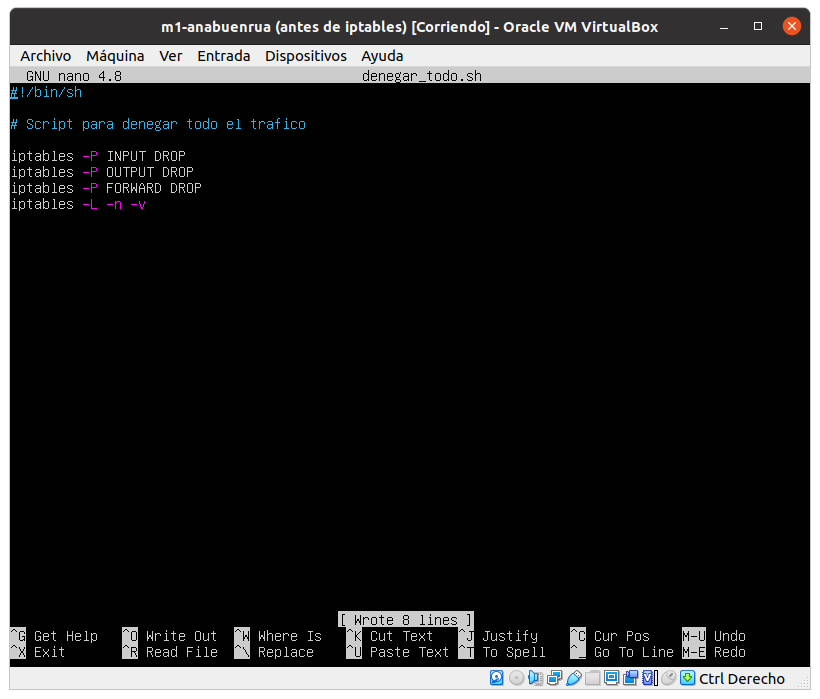
\includegraphics[scale=0.5]{iptable_3}
\end{center}
\end{figure}

Y comprobamos ahora en \eqref{iptable_4} que no podemos acceder a m1 mediante ping.

\begin{figure}[h!]
\begin{center}
\caption{Ping a m1 tras configuración básica de denegar todas las peticiones.}
\label{iptable_4}
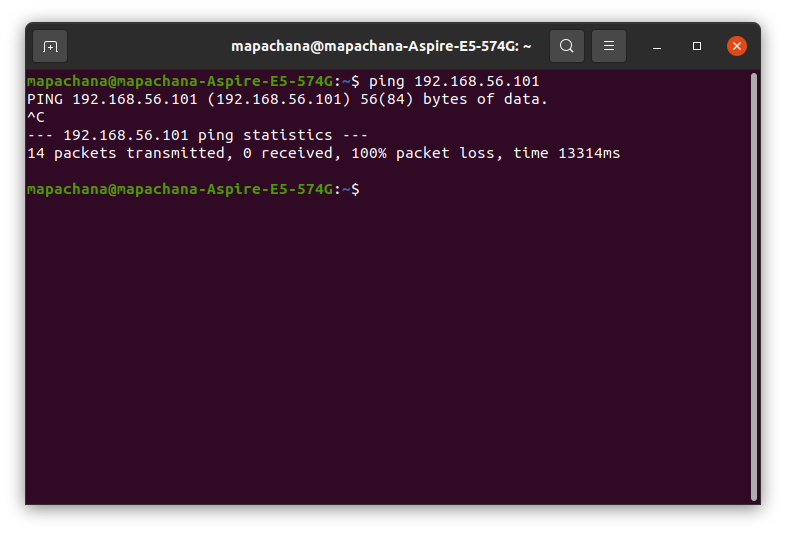
\includegraphics[scale=0.5]{iptable_4}
\end{center}
\end{figure}

\section{Configuración básica}

Vamos a realizar un script con la configuración básica del cortafuegos en todas las máquinas virtuales. Esta configuración va a consistir en denegar todo el tráfico por defecto y solo permitir el tráfico en SSH, HTTP y HTTPS. Al ser un servidor, hay que tener en cuenta que se debe permitir que reciba peticiones.

Dado que la máquina m1 tenía configurado como puerto para ssh el puerto 2022, por simplicidad se ha vuelto a dejar habilitado el puerto 22 para ssh, editando el fichero \verb|/etc/ssh/sshd_config| y cambiando el puerto del 2022 al 22. Para hacer efectiva la configuración se ha relanzado ssh con \verb|sudo systemctl restart ssh|.

El script de configuración básica se muestra  en \eqref{iptable_5}

\begin{figure}[h!]
\begin{center}
\caption{Script de configuración básica para iptables.}
\label{iptable_5}
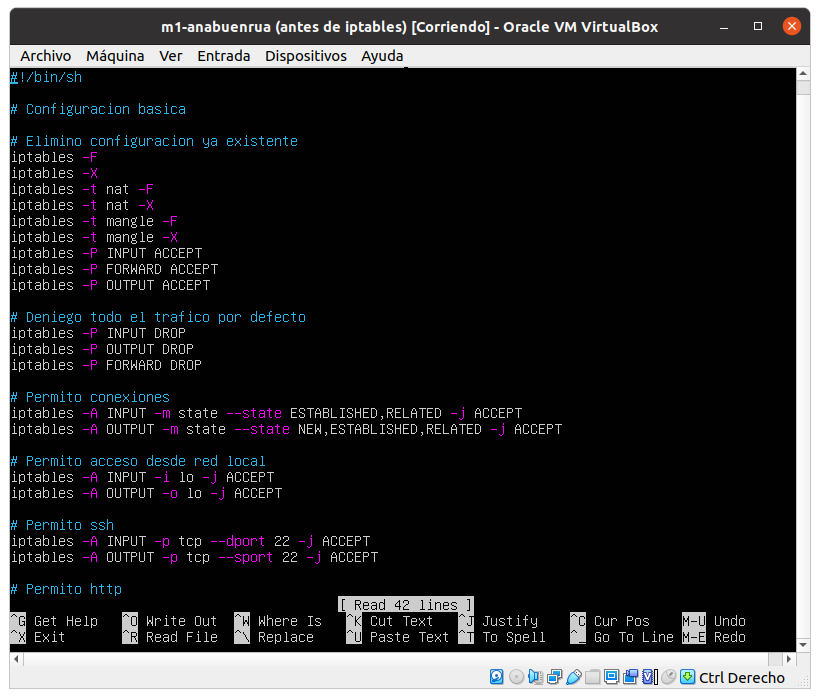
\includegraphics[scale=0.5]{iptable_5}
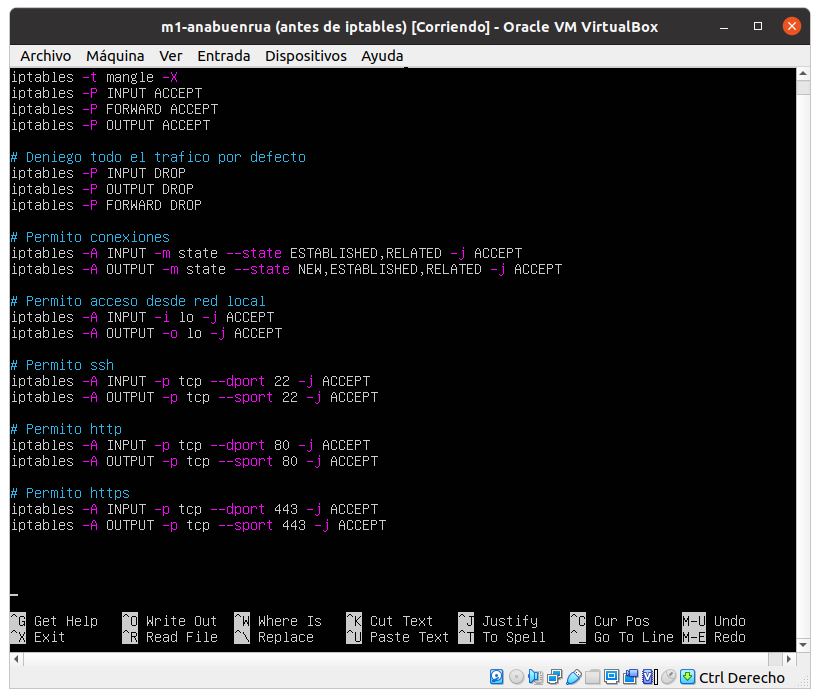
\includegraphics[scale=0.5]{iptable_5a}
\end{center}
\end{figure}

Comprobamos que podemos acceder por http y https a m1, pero no mediante ping en \eqref{iptable_6}.

\begin{figure}[h!]
\begin{center}
\caption{Comprobación de acceso por http y ping a m1 tras configuración básica.}
\label{iptable_6}
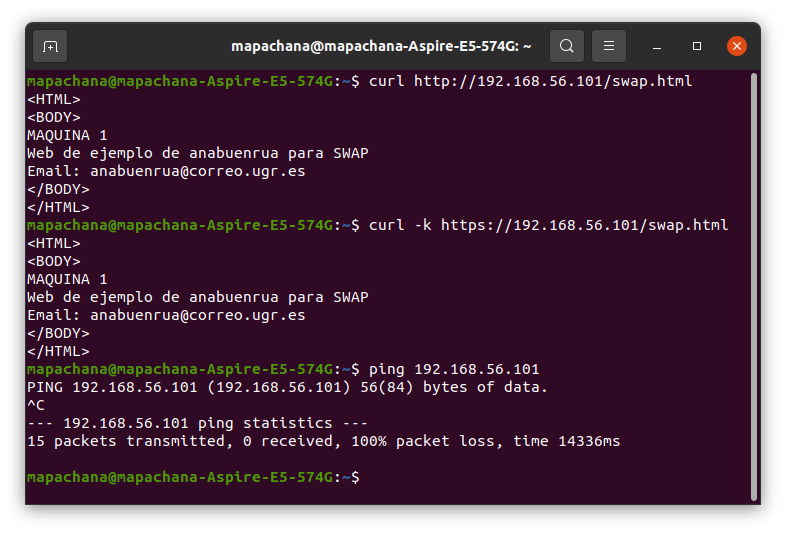
\includegraphics[scale=0.5]{iptable_6}
\end{center}
\end{figure}

Podemos comprobar que m2 y m3 funcionan de igual manera.




\section{Opciones avanzadas}

La configuración anterior se puede mejorar, por ejemplo permitiendo el acceso a m1 y m2 solo a través de m3, además vamos a activar el acceso a ssh, ping y DNS en la red interna.

Para ello, modificamos el script de configuración básica anterior como se muestra en \eqref{iptable_7}

\begin{figure}[h!]
\begin{center}
\caption{Script de configuración avanzada de iptables.}
\label{iptable_7}
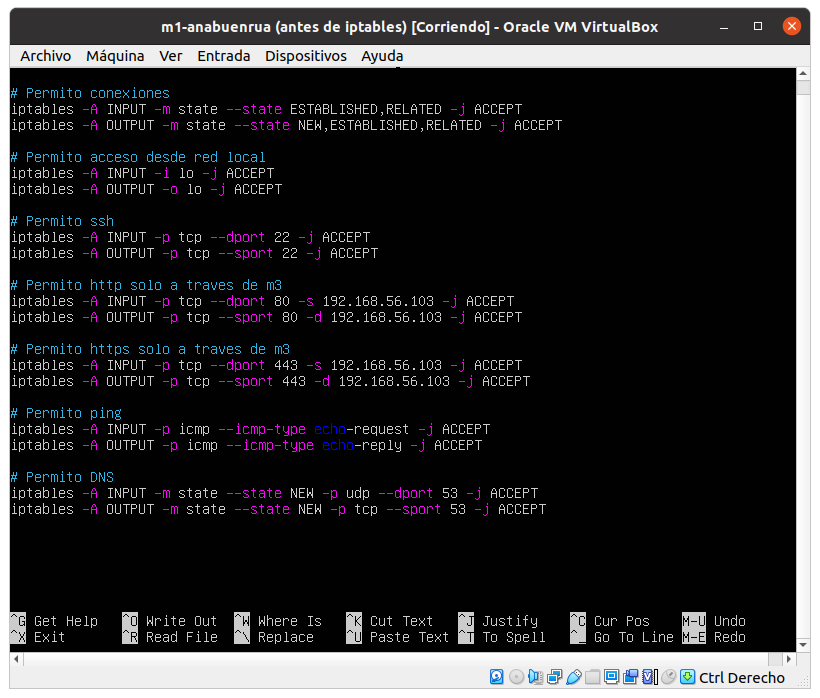
\includegraphics[scale=0.5]{iptable_7}
\end{center}
\end{figure}

Copiamos los scripts a la máquina m2 con scp y comprobamos que la granja funciona correctamente, pues ya no deja acceder a m1 directamente, pero sí mediante m3, como se ve en \eqref{iptable_8}.

\begin{figure}[h!]
\begin{center}
\caption{Prueba de acceso a m1 y m3 mediante http.}
\label{iptable_8}
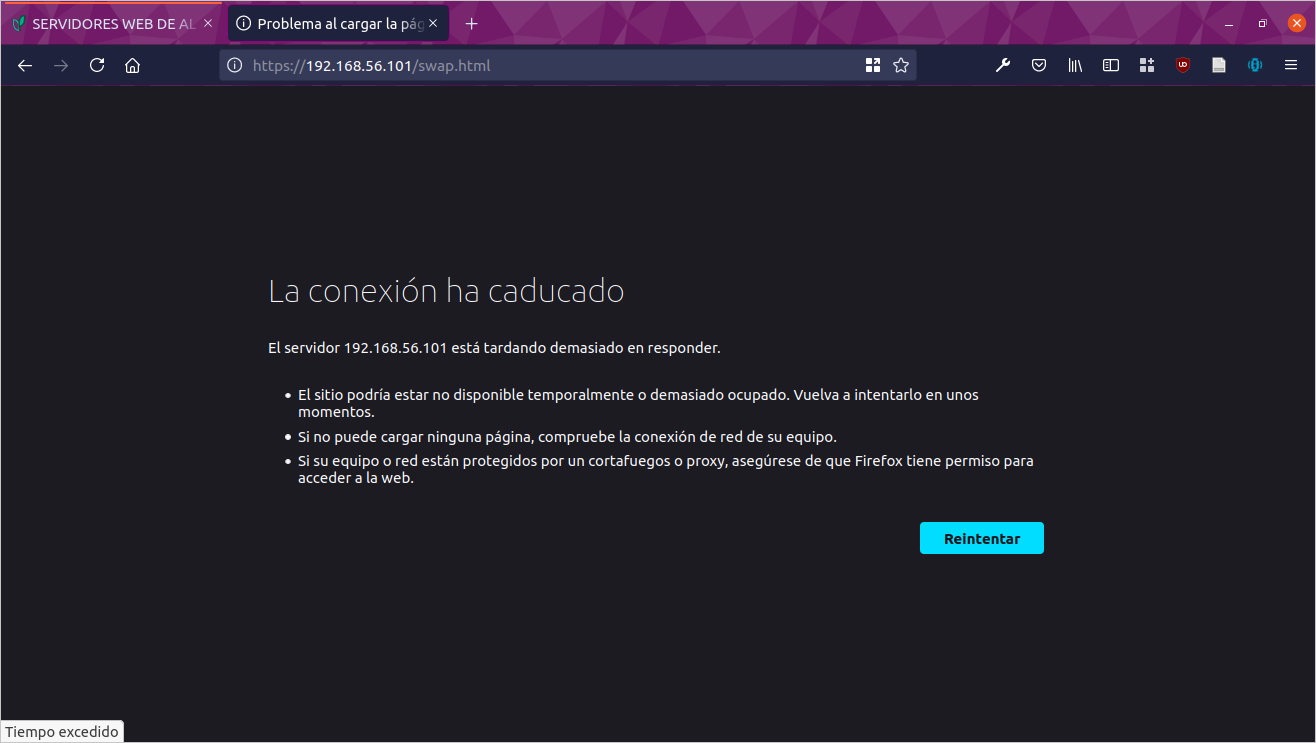
\includegraphics[scale=0.5]{iptable_8}
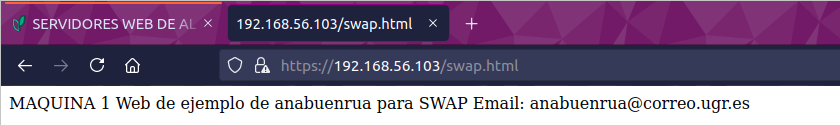
\includegraphics[scale=0.5]{iptable_9}
\end{center}
\end{figure}

Además, ya es posible hacer ping a todas las máquinas como en \eqref{iptable_10}

\begin{figure}[h!]
\begin{center}
\caption{Ping a m1 tras configuración avanzada.}
\label{iptable_10}
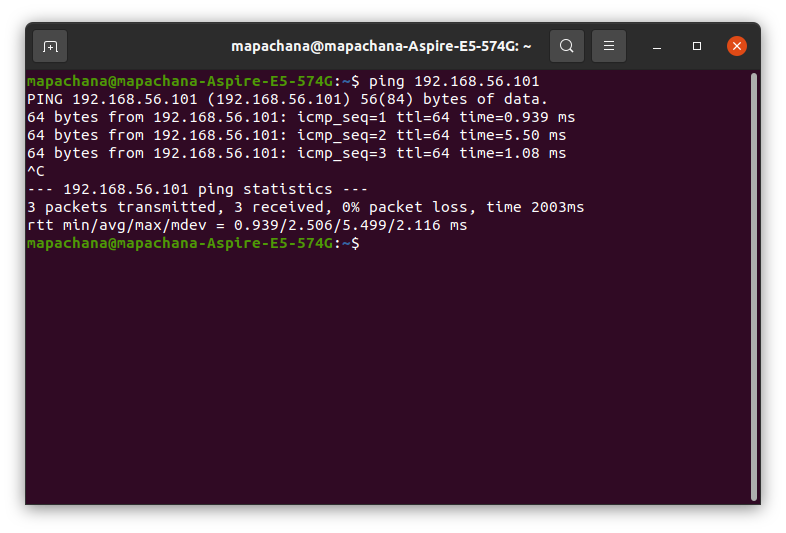
\includegraphics[scale=0.5]{iptable_10}
\end{center}
\end{figure}



\chapter{Configurar cortafuegos al arranque}

Para hacer persistentes las reglas y que se mantengan tras reiniciar las máquinas vamos a instalar \verb|iptables-persistent|. Para ello ejecutamos \eqref{persistent_1}

\begin{figure}[h!]
\begin{center}
\caption{Instañación de iptables-persistent.}
\label{persistent_1}
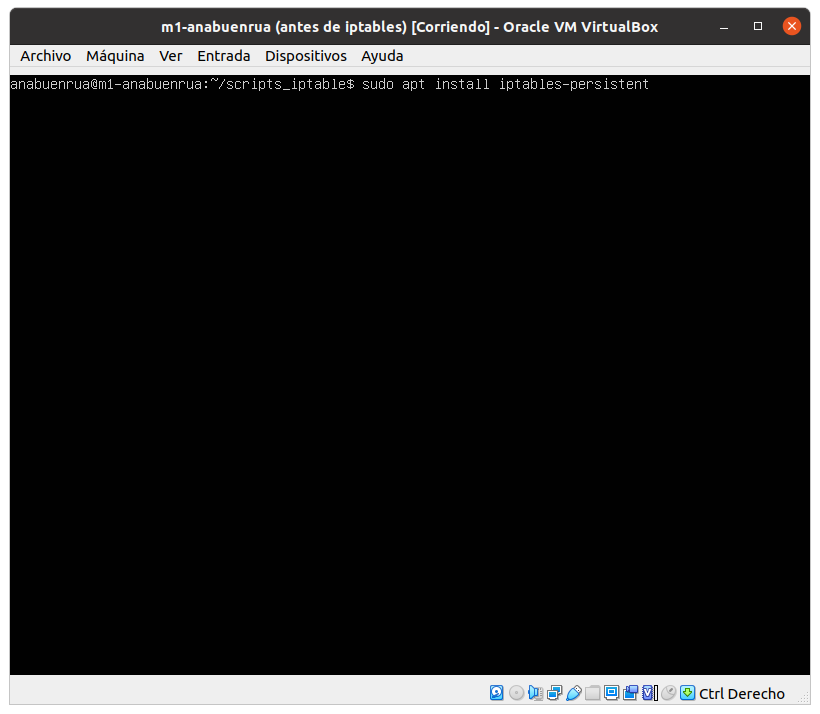
\includegraphics[scale=0.5]{persistent_1}
\end{center}
\end{figure}

Al instalar el paquete, seleccionamos que sí queremos guardar las reglas actuales en los ficheros correspondientes tanto en ip4 como en ip6, como se ve en \eqref{persistent_2}.

\begin{figure}[h!]
\begin{center}
\caption{Copia de reglas tras la instalación de iptables-persisntent.}
\label{persistent_2}
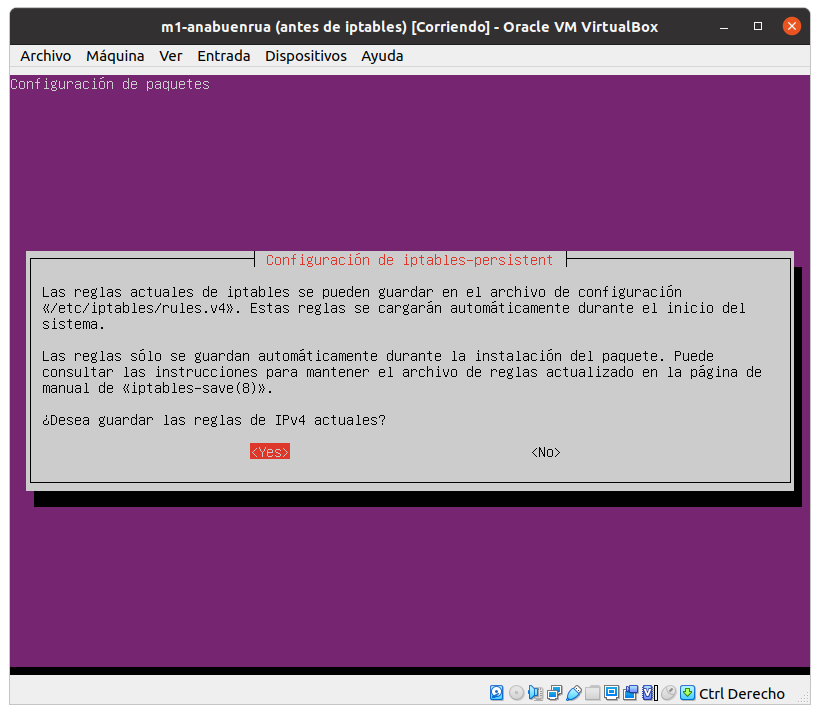
\includegraphics[scale=0.5]{persistent_2}
\end{center}
\end{figure}

El paquete solo guarda las reglas al instalarse, para modificar qué reglas se van a aplicar al reiniciar el sistema, hay que guardarlas ejecutando:

\begin{verbatim}
iptables-save > /etc/iptables/rules.v4
ip6tables-save > /etc/iptables/rules.v6
\end{verbatim}

Probamos a ejecutarlos y comprobamos que hay que loggearse como root para hacerlo, como vemos en \eqref{persistent_3}

\begin{figure}[h!]
\begin{center}
\caption{Modificación de reglas persistentes.}
\label{persistent_3}
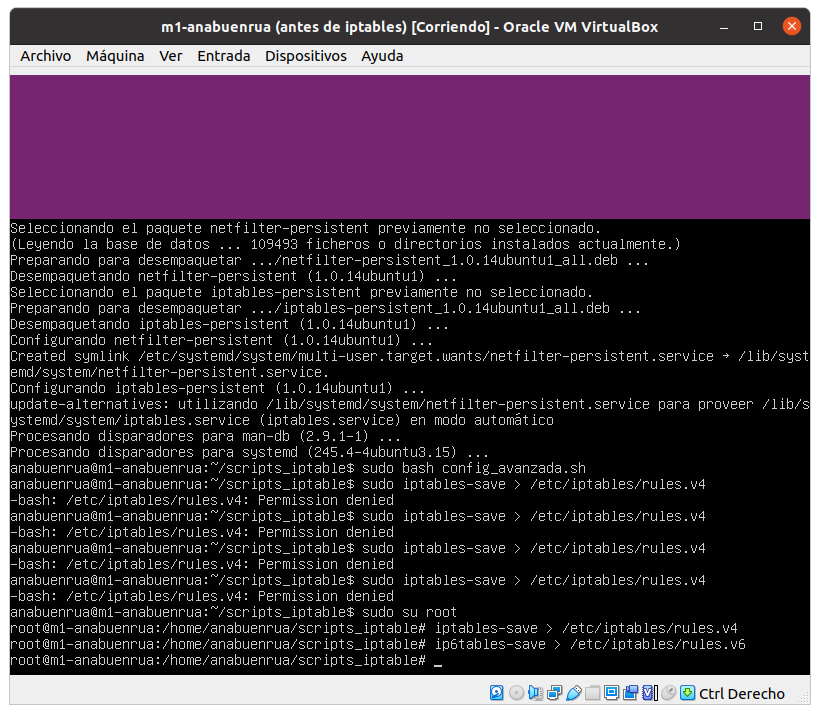
\includegraphics[scale=0.5]{persistent_3}
\end{center}
\end{figure}

Para eliminar la configuración al inicio simplemente borramos los ficheros generados.








\chapter{Certbot}

Vamos a realizar la configuración en m1 y m3, para apache y nginx respectivamente.

\section{Configuración de apache en m1}

Comenzamos instalando en cada una de las máquinas virtuales certbot como se muestra en \eqref{certbot_1}.

\begin{figure}[h!]
\begin{center}
\caption{Instalación de certbot en m1.}
\label{certbot_1}
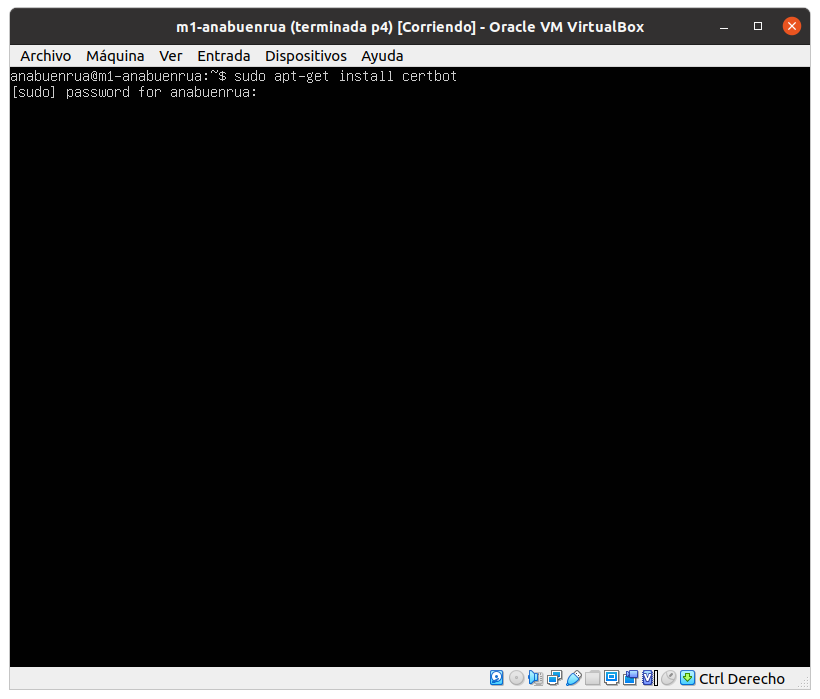
\includegraphics[scale=0.5]{certbot_1}
\end{center}
\end{figure}

En m1 comenzamos instalando el plugin para apache como en \eqref{certbot_2}

\begin{figure}[h!]
\begin{center}
\caption{Instalación del plugin de certbot para apache.}
\label{certbot_2}
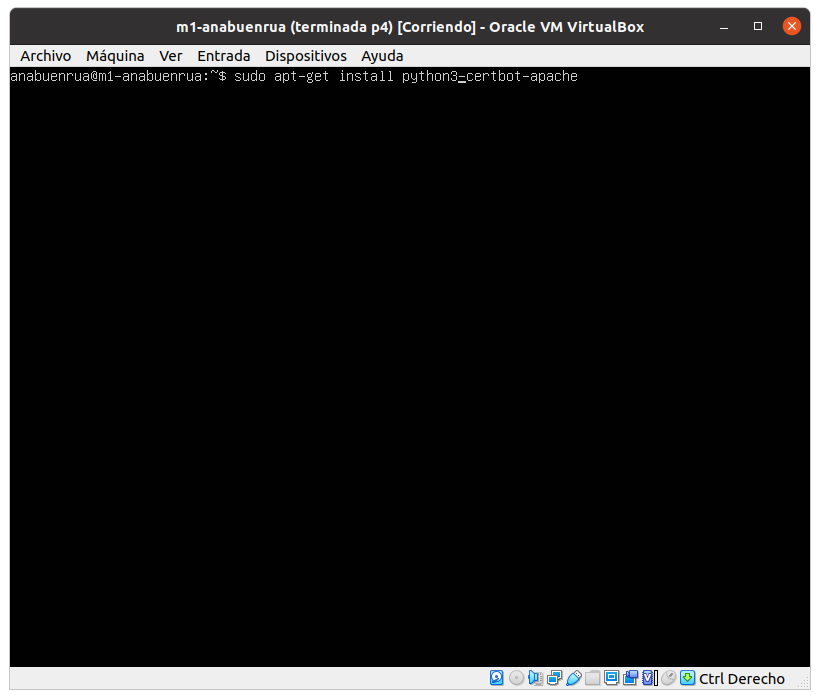
\includegraphics[scale=0.5]{certbot_2}
\end{center}
\end{figure}

Ahora, para instalar un certificado ejecutamos el comando de \eqref{certbot_3} y rellenamos los datos que nos piden.

\begin{figure}[h!]
\begin{center}
\caption{Instalación de cerificado en m1.}
\label{certbot_3}
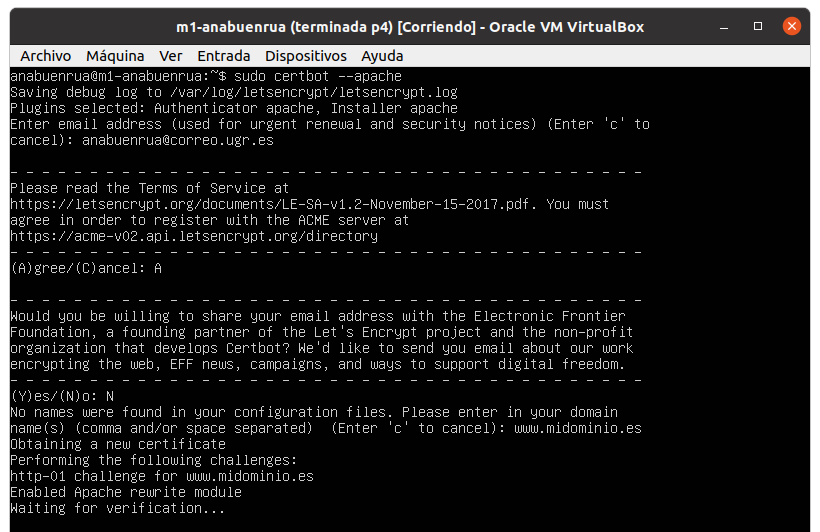
\includegraphics[scale=0.5]{certbot_3}
\end{center}
\end{figure}

Como no tenemos un dominio, el comando anterior nos da el error que se muestra en \eqref{certbot_4}.

\begin{figure}[h!]
\begin{center}
\caption{Error de la instalación de certificado en m1.}
\label{certbot_4}
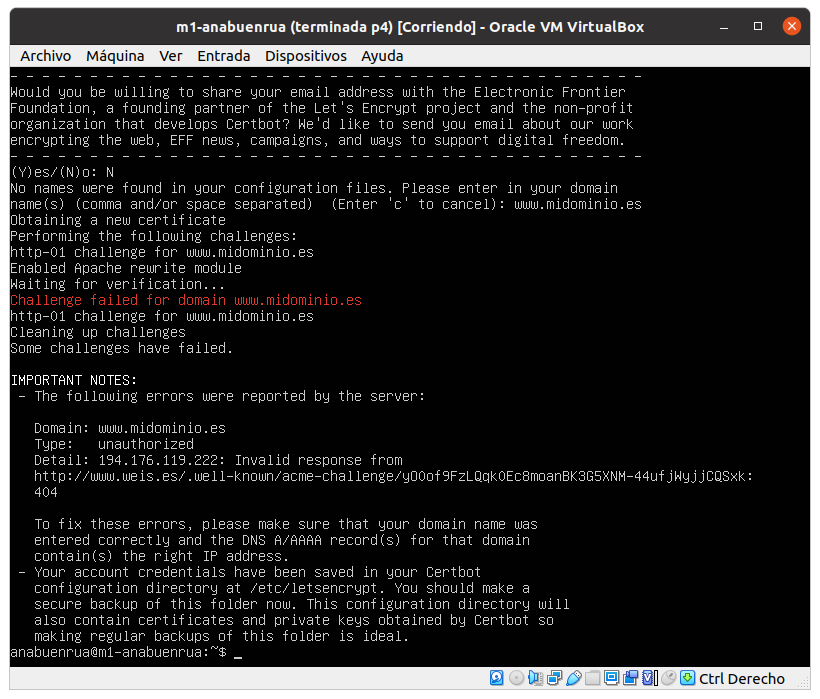
\includegraphics[scale=0.5]{certbot_4}
\end{center}
\end{figure}

Por ello, para solo generar el certificado se ejecuta el comando de \eqref{certbot_5}. Este comando crea el archivo \verb|/etc/cron.d/certbot| de \eqref{certbot_6}.

\begin{figure}[h!]
\begin{center}
\caption{Generación de certificado en m1.}
\label{certbot_5}
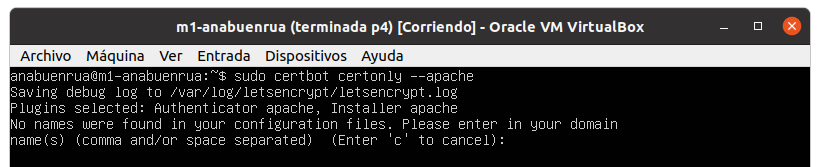
\includegraphics[scale=0.5]{certbot_5}
\end{center}
\end{figure}

\begin{figure}[h!]
\begin{center}
\caption{Archivo /etc/cron.d/certbot}
\label{certbot_6}
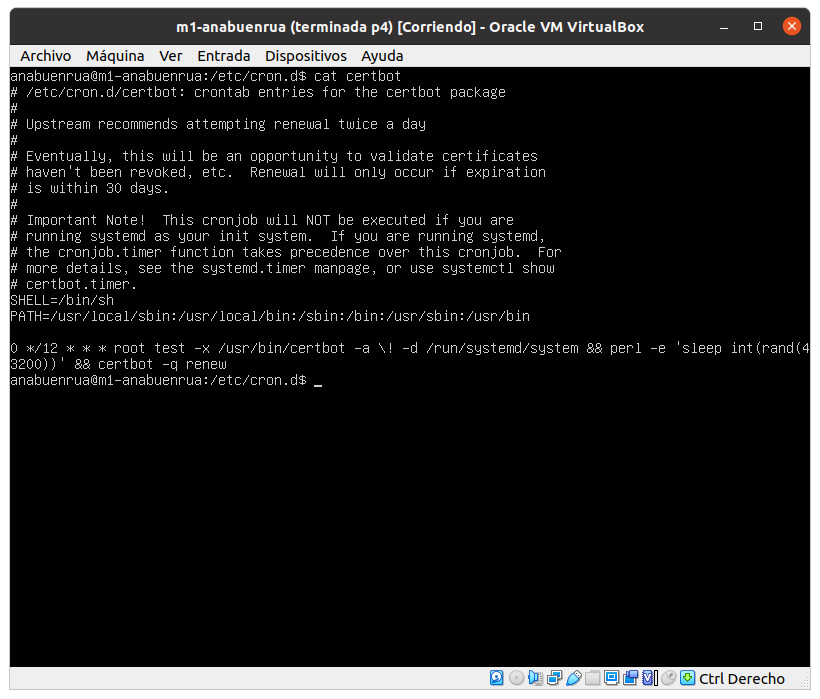
\includegraphics[scale=0.5]{certbot_6}
\end{center}
\end{figure}

\section{Configuración de nginx en m3}

Para realizar la configuración de nginx análogamente se instala el plugin como se ve en \eqref{certbot_7}.

\begin{figure}[h!]
\begin{center}
\caption{Instalación del plugin de certbot para nginx en m3.}
\label{certbot_7}
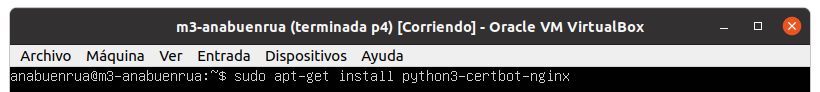
\includegraphics[scale=0.5]{certbot_7}
\end{center}
\end{figure}

De la misma forma ejecutamos el comando de \eqref{certbot_8} rellenando los datos, que nos devuelve el mismo error de antes al no tener dominio.

\begin{figure}[h!]
\begin{center}
\caption{Instalación de certificado en m3.}
\label{certbot_8}
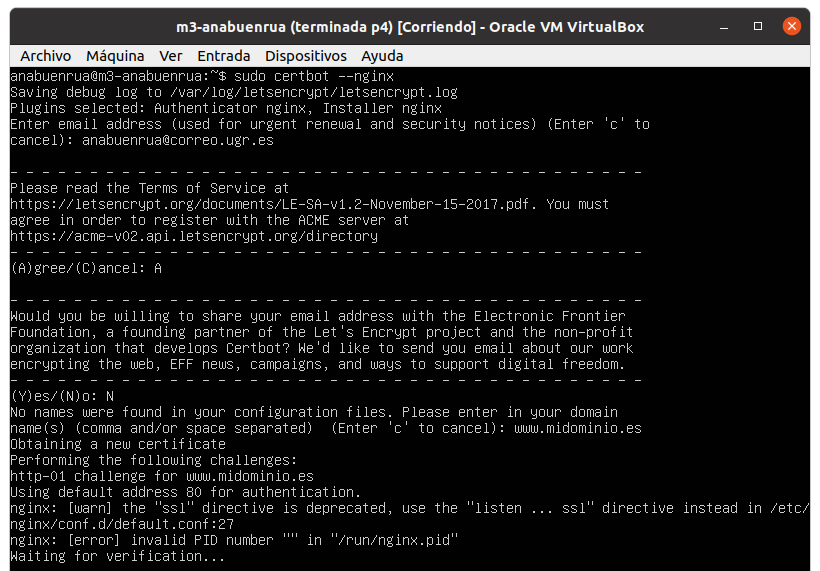
\includegraphics[scale=0.5]{certbot_8}
\end{center}
\end{figure}

Para solamente generar el certificado ejecutamos el comando y rellenamos los datos como en \eqref{certbot_9}.

\begin{figure}[h!]
\begin{center}
\caption{Generación de certificado en m3.}
\label{certbot_9}
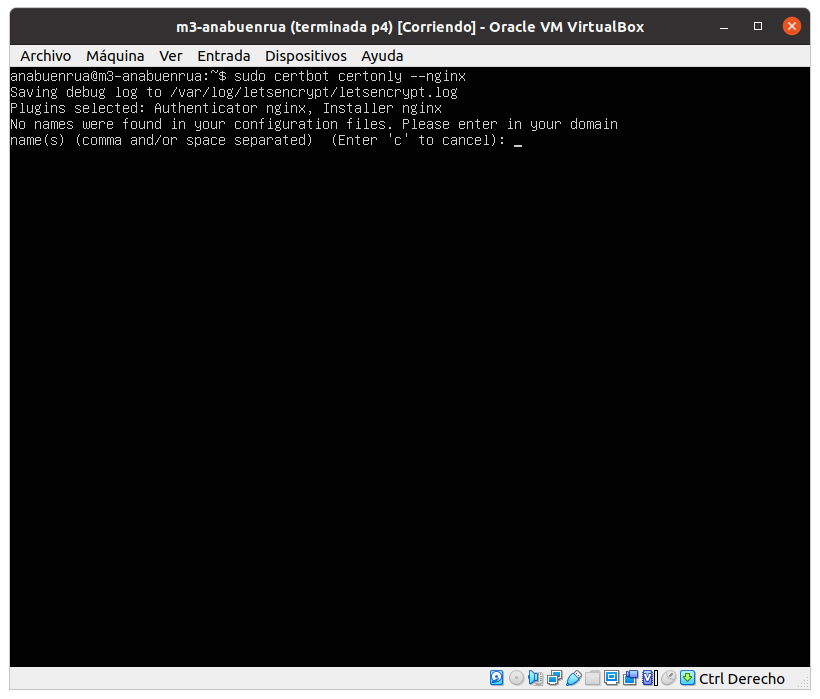
\includegraphics[scale=0.5]{certbot_9}
\end{center}
\end{figure}

